\documentclass{beamer}

% Should be documentclass beamer

\mode<presentation>
{
%  \usetheme[hideothersubsections]{PaloAlto}
  \usetheme{metropolis}
  \setbeamercovered{transparent}
}

\usepackage{amsfonts}
\usepackage{amsmath}
\usepackage{amssymb}
\usepackage{color}
\usepackage{tikz}
\usepackage{pgfplots}
\usepackage{listings}
\usepackage{courier}
%\usepackage[utf8]{inputenc}
%\usepackage[russian]{babel}

\lstset{
  numbers=left,
  basicstyle=\ttfamily\footnotesize,
  numberstyle=\tiny\color{gray},
  stepnumber=1,
  numbersep=10pt,
}

\newcommand{\iu}{\ensuremath{\mathrm{i}}}
\newcommand{\bbR}{\mathbb{R}}
\newcommand{\bbC}{\mathbb{C}}
\newcommand{\calV}{\mathcal{V}}
\newcommand{\calW}{\mathcal{W}}
\newcommand{\macheps}{\epsilon_{\mathrm{mach}}}
\newcommand{\matlab}{\textsc{Matlab}}

\newcommand{\ddiag}{\operatorname{diag}}
\newcommand{\fl}{\operatorname{fl}}
\newcommand{\nnz}{\operatorname{nnz}}
\newcommand{\tr}{\operatorname{tr}}
\renewcommand{\vec}{\operatorname{vec}}

\newcommand{\vertiii}[1]{{\left\vert\kern-0.25ex\left\vert\kern-0.25ex\left\vert #1
    \right\vert\kern-0.25ex\right\vert\kern-0.25ex\right\vert}}
\newcommand{\ip}[2]{\langle #1, #2 \rangle}
\newcommand{\ipx}[2]{\left\langle #1, #2 \right\rangle}
\newcommand{\order}[1]{O( #1 )}

\newcommand{\kron}{\otimes}


\newcommand{\hdr}[2]{
  \title[CS 5220, Fall 2017]{CS 5220: #2}
  \author{David Bindel}
  \date{#1}
}

\pgfdeclarelayer{edgelayer}
\pgfdeclarelayer{nodelayer}
\pgfsetlayers{edgelayer,nodelayer,main}

\hdr{2017-11-14}{Parallel Graph Algorithms}

\begin{document}

\begin{frame}
  \titlepage
\end{frame}

% Graph types and decorations
% Different types of graphs: planar vs small world/power law
% Different types of graph analyses
% What is a ``big'' graph?  Replication as an option
% Fundamental difficulties -- low cost, memory bound, limited BW
% Preprocessing for locality
% Graph data structures and their costs
% Graph algorithms and linear algebra
% Graph BLAS and linear algebra with semirings
% Implicit graphs
% Dynamic graphs
% Parallel graph processing frameworks (including Ligra)
% Fooling the masses + McSherry COST metric

\begin{frame}
  \frametitle{Graphs}

  Mathematically: $G = (V,E)$ where $E \subset V \times V$
  \begin{itemize}
  \item Convention: $|V| = n$ and $|E| = m$
  \item May be directed or undirected
  \item May have weights $w_V : V \rightarrow \bbR$ or
    $w_E : E : \rightarrow \bbR$
  \item May have other node or edge attributes as well
  \item Path is $\left[ \, (u_i,u_{i+1}) \, \right]_{i=1}^\ell \in E^*$,
    sum of weights is length
  \item Diameter is max shortest path length between any $s, t \in V$
  \end{itemize}
  Generalizations:
  \begin{itemize}
  \item Hypergraph (edges in $V^d$)
  \item Multigraph (multiple copies of edges)
  \end{itemize}
\end{frame}

\begin{frame}
  \frametitle{Types of graphs}

  \begin{center}
    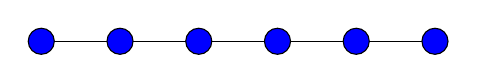
\begin{tikzpicture}
      \draw (0,0) -- (5,0);
      \foreach \x in {0,...,5} {
        \node at (\x, 0) [circle,draw=black,fill=blue] {};
      }      
    \end{tikzpicture}
  \end{center}
\end{frame}

\begin{frame}
  \frametitle{Types of graphs}

  \begin{center}
    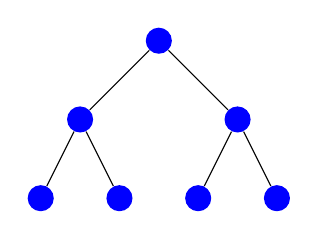
\begin{tikzpicture}
      \node(r)  at (0,0) [circle,fill=blue] {};
      \node(r0) at (-1,-1) [circle,fill=blue] {};
      \node(r1) at ( 1,-1) [circle,fill=blue] {};
      \node(r00) at (-1.5,-2) [circle,fill=blue] {};
      \node(r01) at (-0.5,-2) [circle,fill=blue] {};
      \node(r10) at ( 0.5,-2) [circle,fill=blue] {};
      \node(r11) at ( 1.5,-2) [circle,fill=blue] {};
      \draw (r) -- (r0);
      \draw (r) -- (r1);
      \draw (r0) -- (r00);
      \draw (r0) -- (r01);
      \draw (r1) -- (r10);
      \draw (r1) -- (r11);
    \end{tikzpicture}
  \end{center}
\end{frame}

\begin{frame}
  \frametitle{Types of graphs}

  \begin{center}
    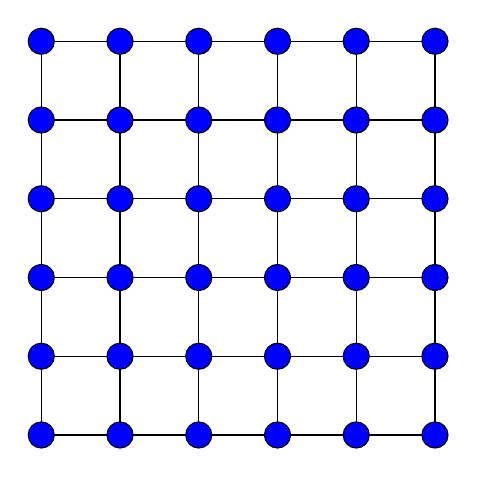
\begin{tikzpicture}
      \draw (0,0) grid (5,5);
      \foreach \x in {0,...,5}
      \foreach \y in {0,...,5} {
        \node at (\x, \y) [circle,draw=black,fill=blue] {};
      }      
    \end{tikzpicture}
  \end{center}
\end{frame}

\begin{frame}
  \frametitle{Types of graphs}

  \begin{center}
    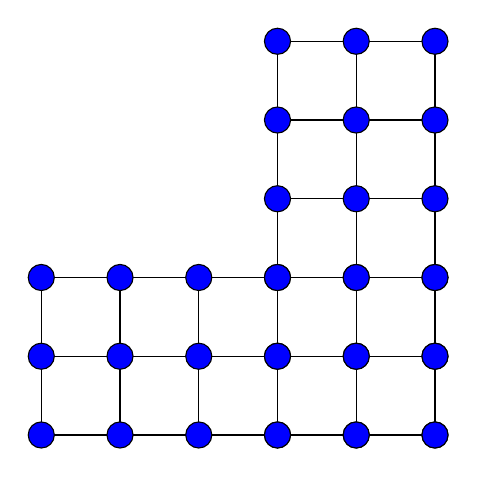
\begin{tikzpicture}
      \draw (0,0) grid (5,2);
      \draw (3,0) grid (5,5);
      \foreach \x in {0,...,5}
      \foreach \y in {0,...,2} {
        \node at (\x, \y) [circle,draw=black,fill=blue] {};
      }      
      \foreach \x in {3,...,5}
      \foreach \y in {0,...,5} {
        \node at (\x, \y) [circle,draw=black,fill=blue] {};
      }      
    \end{tikzpicture}
  \end{center}
\end{frame}

\begin{frame}
  \frametitle{Types of graphs}

  \begin{center}
    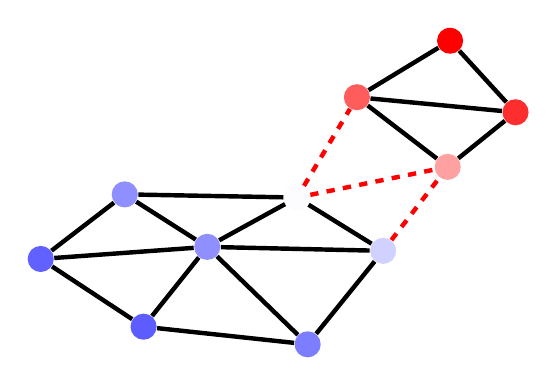
\begin{tikzpicture}
      \node (n1) at (1.108060,0.168294) [circle,fill=blue!64] {};
\node (n2) at (1.916771,1.181859) [circle,fill=blue!44] {};
\node (n3) at (-0.197998,1.028224) [circle,fill=blue!62] {};
\node (n4) at (0.869271,1.848640) [circle,fill=blue!44] {};
\node (n5) at (3.056732,1.808215) [circle,fill=blue!1] {};
\node (n6) at (3.192034,-0.055883) [circle,fill=blue!51] {};
\node (n7) at (4.150780,1.131397) [circle,fill=blue!18] {};
\node (n8) at (4.970900,2.197872) [circle,fill=red!37] {};
\node (n9) at (3.817774,3.082424) [circle,fill=red!64] {};
\node (n10) at (5.832186,2.891196) [circle,fill=red!82] {};
\node (n11) at (5.000885,3.800002) [circle,fill=red!100] {};
\draw[    ultra thick       ] (n1) -- (n2);
\draw[    ultra thick       ] (n1) -- (n3);
\draw[    ultra thick       ] (n1) -- (n6);
\draw[    ultra thick       ] (n2) -- (n3);
\draw[    ultra thick       ] (n2) -- (n4);
\draw[    ultra thick       ] (n2) -- (n5);
\draw[    ultra thick       ] (n2) -- (n6);
\draw[    ultra thick       ] (n2) -- (n7);
\draw[    ultra thick       ] (n3) -- (n4);
\draw[    ultra thick       ] (n4) -- (n5);
\draw[    ultra thick       ] (n5) -- (n7);
\draw[red,ultra thick,dashed] (n5) -- (n8);
\draw[red,ultra thick,dashed] (n5) -- (n9);
\draw[    ultra thick       ] (n6) -- (n7);
\draw[red,ultra thick,dashed] (n7) -- (n8);
\draw[    ultra thick       ] (n8) -- (n9);
\draw[    ultra thick       ] (n8) -- (n10);
\draw[    ultra thick       ] (n9) -- (n10);
\draw[    ultra thick       ] (n9) -- (n11);
\draw[    ultra thick       ] (n10) -- (n11);

    \end{tikzpicture}
  \end{center}
\end{frame}

\begin{frame}
  \frametitle{Types of graphs}

  \begin{center}
    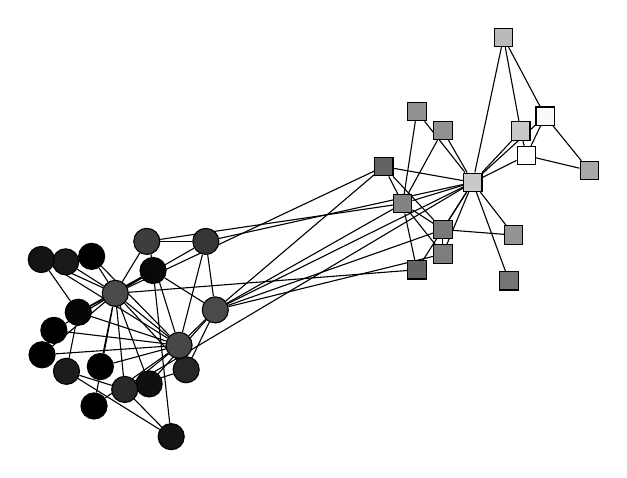
\begin{tikzpicture}[scale=0.5]
  \begin{pgfonlayer}{nodelayer}
    \node [rectangle,fill=black!21,draw=black] (1) at (11.560000, -4.280000) {};
    \node [rectangle,fill=black!49,draw=black] (2) at (9.780000, -4.820000) {};
    \node [circle,fill=black!71,draw=black] (3) at (5.020000, -7.520000) {};
    \node [rectangle,fill=black!53,draw=black] (4) at (10.800000, -5.480000) {};
    \node [rectangle,fill=black!21,draw=black] (5) at (12.780000, -2.980000) {};
    \node [rectangle,fill=black!2,draw=black] (6) at (13.400000, -2.600000) {};
    \node [rectangle,fill=black!0,draw=black] (7) at (12.920000, -3.600000) {};
    \node [rectangle,fill=black!51,draw=black] (8) at (10.800000, -6.100000) {};
    \node [circle,fill=black!79,draw=black] (9) at (4.780000, -5.780000) {};
    \node [circle,fill=black!94,draw=black] (10) at (3.340000, -9.400000) {};
    \node [rectangle,fill=black!27,draw=black] (11) at (12.340000, -0.600000) {};
    \node [rectangle,fill=black!54,draw=black] (12) at (12.480000, -6.780000) {};
    \node [rectangle,fill=black!42,draw=black] (13) at (12.600000, -5.620000) {};
    \node [rectangle,fill=black!61,draw=black] (14) at (9.300000, -3.880000) {};
    \node [circle,fill=black!100,draw=black] (15) at (2.100000, -8.960000) {};
    \node [circle,fill=black!100,draw=black] (16) at (1.880000, -6.160000) {};
    \node [rectangle,fill=black!34,draw=black] (17) at (14.520000, -3.980000) {};
    \node [rectangle,fill=black!43,draw=black] (18) at (10.140000, -2.480000) {};
    \node [circle,fill=black!100,draw=black] (19) at (1.940000, -9.960000) {};
    \node [rectangle,fill=black!61,draw=black] (20) at (10.140000, -6.500000) {};
    \node [circle,fill=black!100,draw=black] (21) at (0.620000, -8.660000) {};
    \node [rectangle,fill=black!43,draw=black] (22) at (10.800000, -2.960000) {};
    \node [circle,fill=black!100,draw=black] (23) at (0.920000, -8.040000) {};
    \node [circle,fill=black!98,draw=black] (24) at (1.540000, -7.580000) {};
    \node [circle,fill=black!92,draw=black] (25) at (3.900000, -10.740000) {};
    \node [circle,fill=black!89,draw=black] (26) at (1.240000, -9.080000) {};
    \node [circle,fill=black!90,draw=black] (27) at (1.220000, -6.300000) {};
    \node [circle,fill=black!97,draw=black] (28) at (3.440000, -6.520000) {};
    \node [circle,fill=black!85,draw=black] (29) at (4.280000, -9.040000) {};
    \node [circle,fill=black!92,draw=black] (30) at (0.600000, -6.240000) {};
    \node [circle,fill=black!76,draw=black] (31) at (3.280000, -5.780000) {};
    \node [circle,fill=black!84,draw=black] (32) at (2.720000, -9.540000) {};
    \node [circle,fill=black!72,draw=black] (33) at (4.100000, -8.420000) {};
    \node [circle,fill=black!71,draw=black] (34) at (2.480000, -7.100000) {};
  \end{pgfonlayer}
  \begin{pgfonlayer}{edgelayer}
    \draw (2) to (1);
    \draw (3) to (1);
    \draw (3) to (2);
    \draw (4) to (1);
    \draw (4) to (2);
    \draw (4) to (3);
    \draw (5) to (1);
    \draw (6) to (1);
    \draw (7) to (1);
    \draw (7) to (5);
    \draw (7) to (6);
    \draw (8) to (1);
    \draw (8) to (2);
    \draw (8) to (3);
    \draw (8) to (4);
    \draw (9) to (1);
    \draw (9) to (3);
    \draw (10) to (3);
    \draw (11) to (1);
    \draw (11) to (5);
    \draw (11) to (6);
    \draw (12) to (1);
    \draw (13) to (1);
    \draw (13) to (4);
    \draw (14) to (1);
    \draw (14) to (2);
    \draw (14) to (3);
    \draw (14) to (4);
    \draw (17) to (6);
    \draw (17) to (7);
    \draw (18) to (1);
    \draw (18) to (2);
    \draw (20) to (1);
    \draw (20) to (2);
    \draw (22) to (1);
    \draw (22) to (2);
    \draw (26) to (24);
    \draw (26) to (25);
    \draw (28) to (3);
    \draw (28) to (24);
    \draw (28) to (25);
    \draw (29) to (3);
    \draw (30) to (24);
    \draw (30) to (27);
    \draw (31) to (2);
    \draw (31) to (9);
    \draw (32) to (1);
    \draw (32) to (25);
    \draw (32) to (26);
    \draw (32) to (29);
    \draw (33) to (3);
    \draw (33) to (9);
    \draw (33) to (15);
    \draw (33) to (16);
    \draw (33) to (19);
    \draw (33) to (21);
    \draw (33) to (23);
    \draw (33) to (24);
    \draw (33) to (30);
    \draw (33) to (31);
    \draw (33) to (32);
    \draw (34) to (9);
    \draw (34) to (10);
    \draw (34) to (14);
    \draw (34) to (15);
    \draw (34) to (16);
    \draw (34) to (19);
    \draw (34) to (20);
    \draw (34) to (21);
    \draw (34) to (23);
    \draw (34) to (24);
    \draw (34) to (27);
    \draw (34) to (28);
    \draw (34) to (29);
    \draw (34) to (30);
    \draw (34) to (31);
    \draw (34) to (32);
    \draw (34) to (33);
  \end{pgfonlayer}
\end{tikzpicture}

  \end{center}
\end{frame}

\begin{frame}
  \frametitle{Types of graphs}

  Many possible structures:
  \begin{itemize}
  \item Lines and trees
  \item Completely regular grids
  \item Planar graphs (no edges need cross)
  \item Low-dimensional Euclidean
  \item Power law graphs
  \item ...
  \end{itemize}
  Algorithms are not one-size-fits-all!
\end{frame}

\begin{frame}
  \frametitle{Ends of a spectrum}

  \begin{center}
    \begin{tabular}{r|l|l}
      & Planar & Power law \\ \hline
      Vertex degree & Uniformly small &
      $P(\mathrm{deg} = k) \sim k^{-\gamma}$ \\
      Radius & $\Omega(\sqrt{n})$ & Small \\
      Edge separators & $O(\sqrt{n})$ & nothing small \\
      Linear solve & Direct OK & Iterative \\
      Prototypical apps & PDEs & Social networks
    \end{tabular}

    \vspace{1cm}
    Calls for different methods!
  \end{center}
\end{frame}

\begin{frame}
  \frametitle{Applications: Routing and shortest paths}

  \begin{center}
    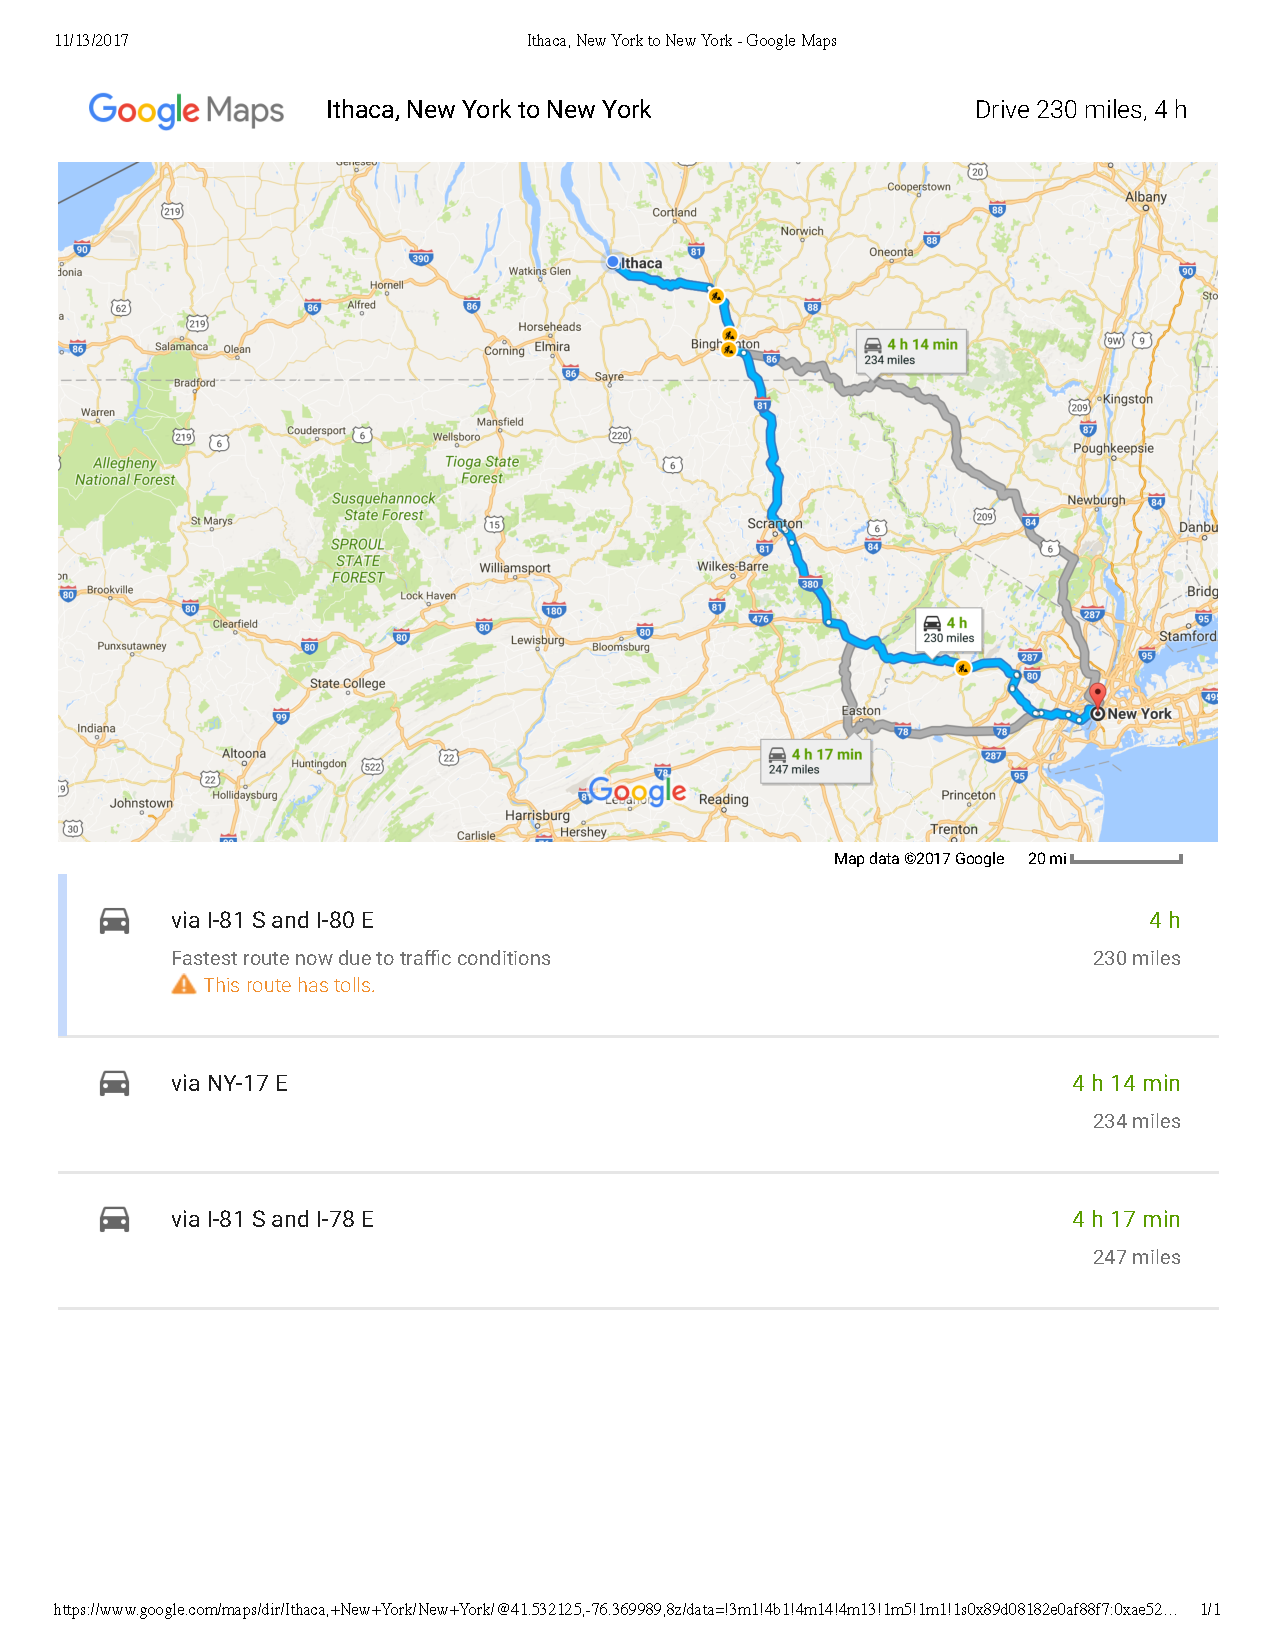
\includegraphics[width=0.5\textwidth]{figs/ithaca2nyc.pdf}
  \end{center}
\end{frame}

\begin{frame}
  \frametitle{Applications: Traversal, ranking, clustering}

  \begin{center}
    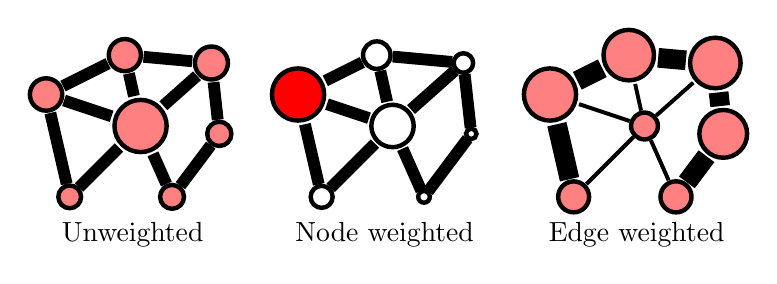
\begin{tikzpicture}[scale=0.4]

\begin{scope}
\node [draw,circle,scale=1.240864,ultra thick,fill=red!50] (1) at (-3.500000, 1.250000) {};
\node [draw,circle,scale=1.231051,ultra thick,fill=red!50] (2) at (-1.000000, 2.500000) {};
\node [draw,circle,scale=0.872732,ultra thick,fill=red!50] (3) at (-2.750000, -2.000000) {};
\node [draw,circle,scale=0.928713,ultra thick,fill=red!50] (4) at (2.000000, 0.000000) {};
\node [draw,circle,scale=1.264655,ultra thick,fill=red!50] (5) at (1.750000, 2.250000) {};
\node [draw,circle,scale=0.915857,ultra thick,fill=red!50] (6) at (0.500000, -2.000000) {};
\node [draw,circle,scale=2.000000,ultra thick,fill=red!50] (7) at (-0.500000, 0.250000) {};
\draw [line width=1.500000 mm] (1) to (2);
\draw [line width=1.500000 mm] (1) to (3);
\draw [line width=1.500000 mm] (2) to (5);
\draw [line width=1.500000 mm] (4) to (5);
\draw [line width=1.500000 mm] (4) to (6);
\draw [line width=1.500000 mm] (1) to (7);
\draw [line width=1.500000 mm] (2) to (7);
\draw [line width=1.500000 mm] (3) to (7);
\draw [line width=1.500000 mm] (5) to (7);
\draw [line width=1.500000 mm] (6) to (7);
\node [below,align=center] at (-0.75,-2.5) {Unweighted};
\end{scope}

\begin{scope}[xshift=8cm]
\node [draw,circle,scale=2.000000,ultra thick,fill=red!100] (1) at (-3.500000, 1.250000) {};
\node [draw,circle,scale=1.053931,ultra thick,fill=red!0] (2) at (-1.000000, 2.500000) {};
\node [draw,circle,scale=0.842809,ultra thick,fill=red!0] (3) at (-2.750000, -2.000000) {};
\node [draw,circle,scale=0.400894,ultra thick,fill=red!0] (4) at (2.000000, 0.000000) {};
\node [draw,circle,scale=0.745137,ultra thick,fill=red!0] (5) at (1.750000, 2.250000) {};
\node [draw,circle,scale=0.446523,ultra thick,fill=red!0] (6) at (0.500000, -2.000000) {};
\node [draw,circle,scale=1.624369,ultra thick,fill=red!0] (7) at (-0.500000, 0.250000) {};
\draw [line width=1.500000 mm] (1) to (2);
\draw [line width=1.500000 mm] (1) to (3);
\draw [line width=1.500000 mm] (2) to (5);
\draw [line width=1.500000 mm] (4) to (5);
\draw [line width=1.500000 mm] (4) to (6);
\draw [line width=1.500000 mm] (1) to (7);
\draw [line width=1.500000 mm] (2) to (7);
\draw [line width=1.500000 mm] (3) to (7);
\draw [line width=1.500000 mm] (5) to (7);
\draw [line width=1.500000 mm] (6) to (7);
\node [below,align=center] at (-0.75,-2.5) {Node weighted};
\end{scope}

\begin{scope}[xshift=16cm]
\node [draw,circle,scale=2.000000,ultra thick,fill=red!50] (1) at (-3.500000, 1.250000) {};
\node [draw,circle,scale=1.934370,ultra thick,fill=red!50] (2) at (-1.000000, 2.500000) {};
\node [draw,circle,scale=1.185575,ultra thick,fill=red!50] (3) at (-2.750000, -2.000000) {};
\node [draw,circle,scale=1.830214,ultra thick,fill=red!50] (4) at (2.000000, 0.000000) {};
\node [draw,circle,scale=1.938059,ultra thick,fill=red!50] (5) at (1.750000, 2.250000) {};
\node [draw,circle,scale=1.190689,ultra thick,fill=red!50] (6) at (0.500000, -2.000000) {};
\node [draw,circle,scale=1.028430,ultra thick,fill=red!50] (7) at (-0.500000, 0.250000) {};
\draw [line width=2.500000 mm] (1) to (2);
\draw [line width=2.500000 mm] (1) to (3);
\draw [line width=2.500000 mm] (2) to (5);
\draw [line width=2.500000 mm] (4) to (5);
\draw [line width=2.500000 mm] (4) to (6);
\draw [line width=0.500000 mm] (1) to (7);
\draw [line width=0.500000 mm] (2) to (7);
\draw [line width=0.500000 mm] (3) to (7);
\draw [line width=0.500000 mm] (5) to (7);
\draw [line width=0.500000 mm] (6) to (7);
\node [below,align=center] at (-0.75,-2.5) {Edge weighted};
\end{scope}

\end{tikzpicture}
  \end{center}

  \begin{itemize}
    \item Web crawl / traversal
    \item PageRank, HITS
    \item Clustering similar documents
  \end{itemize}
\end{frame}

\begin{frame}
  \frametitle{Applications: Sparse solvers}

  \begin{center}
    \href{http://yifanhu.net/GALLERY/GRAPHS/GIF_SMALL/Pothen@barth5.html}{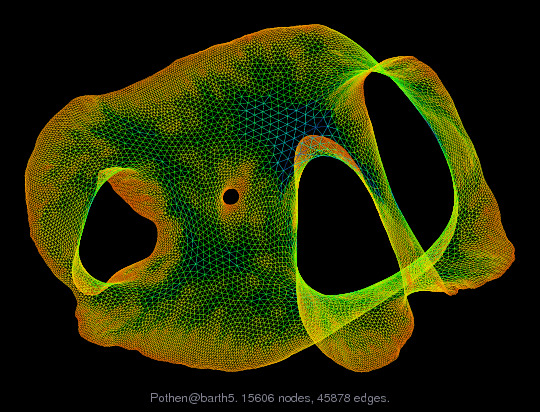
\includegraphics[width=0.5\textwidth]{figs/Pothen-barth5.jpg}}
  \end{center}

  \begin{itemize}
  \item Ordering for sparse factorization
  \item Partitioning
  \item Graph coarsening for AMG
  \item Other preconditioning ops...
  \end{itemize}
\end{frame}

\begin{frame}
  \frametitle{Applications: Dimensionality reduction}

  \begin{center}
    \href{http://web.mit.edu/cocosci/isomap/isomap.html}{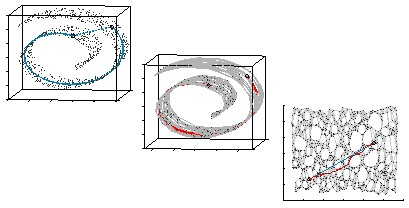
\includegraphics[width=0.8\textwidth]{figs/web1.jpg}}
  \end{center}
\end{frame}

\begin{frame}
  \frametitle{Common building blocks}

  \begin{itemize}
  \item Traversals
  \item Shortest paths
  \item Spanning tree
  \item Flow computations
  \item Topological sort
  \item Coloring
  \item ...
  \end{itemize}
  ... and most of sparse linear algebra.
\end{frame}

\begin{frame}
  \frametitle{Over-simple models}

    \begin{center}
    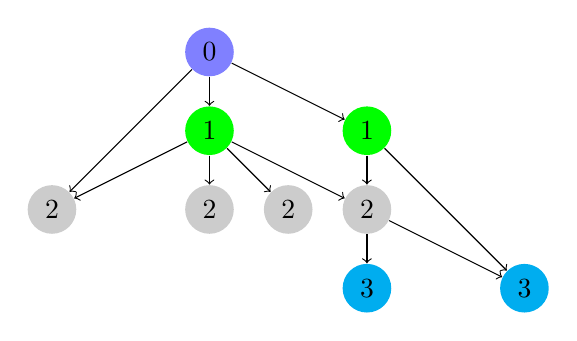
\begin{tikzpicture}
      \node (n0) at (-1,0) [circle,fill=blue!50] {$0$};
      \node (n1) at (-1,-1) [circle,fill=green] {$1$};
      \node (n2) at ( 1,-1) [circle,fill=green] {$1$};
      \node (n3) at (-3,-2) [circle,fill=black!20] {$2$};
      \node (n4) at (-1,-2) [circle,fill=black!20] {$2$};
      \node (n5) at ( 0,-2) [circle,fill=black!20] {$2$};
      \node (n6) at ( 1,-2) [circle,fill=black!20] {$2$};
      \node (n7) at ( 1,-3) [circle,fill=cyan] {$3$};
      \node (n8) at ( 3,-3) [circle,fill=cyan] {$3$};
      \draw[->] (n0) -- (n1);
      \draw[->] (n0) -- (n2);
      \draw[->] (n0) -- (n3);
      \draw[->] (n1) -- (n3);
      \draw[->] (n1) -- (n4);
      \draw[->] (n1) -- (n5);
      \draw[->] (n1) -- (n6);
      \draw[->] (n2) -- (n6);
      \draw[->] (n6) -- (n7);
      \draw[->] (n6) -- (n8);
      \draw[->] (n2) -- (n8);
    \end{tikzpicture}
    \end{center}
    Let $t_p = $ idealized time on $p$ processors
    \begin{itemize}
    \item $t_1 = $ work
    \item $t_\infty = $ span (or depth, or critical path length)
    \end{itemize}

\end{frame}

\begin{frame}
  \frametitle{One implication}

  Don't bother with parallel DFS!  Span is $\Omega(n)$. \\
  Let's spend a few minutes on more productive algorithms...
\end{frame}

\begin{frame}
  \frametitle{Parallel BFS}

  Simple idea: parallelize across frontiers
  \begin{itemize}
  \item Pro: Simple to think about
  \item Pro: Lots of parallelism with small radius?
  \item Con: What if frontiers are small?
  \end{itemize}
\end{frame}

\begin{frame}
  \frametitle{Parallel BFS: Ullman-Yannakakis}

  Assuming a high-diameter graph:
  \begin{itemize}
  \item Form set $S$ with start + random nodes, $|S| = \Theta(\sqrt{n}
    \log n)$ --- long shortest paths must go through $S$ with high prob
  \item Take $\sqrt{n}$ steps of BFS from each seed in $S$
  \item Form aux weighted graph for distances between seeds
  \item Run all-pairs shortest path on aux graph
  \end{itemize}
  OK, but what if diameter is not large?
  
\end{frame}

\begin{frame}
  \frametitle{LA take}

  \begin{itemize}
  \item Indicate frontier at each stage by $x$
  \item $x' = A^T x$ (multiply=select, add=min)
  \end{itemize}
\end{frame}

\begin{frame}
  \frametitle{Parallel BFS: LA perspective}

  Key ideas:
  \begin{itemize}
  \item At some point, switch from top-down expanding frontier (``are you my
    child?'') to bottom-up checking for parents (``are you my parent?'')
  \item Use 2D blocking of adjacency
  \item Temporally partition work: vertex processed by at most one
    processor at a time, cycle processors (``systolic rotation'')
  \end{itemize}
  Together gives state-of-art performance.  But...
\end{frame}

\begin{frame}
  \frametitle{Single-source shortest path}

  Classic algorithm: Dijkstra
  \begin{itemize}
  \item Dequeue closest point from frontier and expand frontier
  \item Update priority queue of distances (can be done in parallel)
  \item Repeat
  \end{itemize}
  Or run serial Dijkstra from different sources for APSP.
\end{frame}

\begin{frame}
  \frametitle{Alternate idea: label correcting}

  Initialize $d[u]$ with distance over-estimates to source
  \begin{itemize}
  \item $d[s] = 0$
  \item Repeatedly relax $d[u] := \min_{(v,u) \in E} d[v] + w(v,u)$
  \end{itemize}
  Converges (eventually) as long as all nodes visited repeatedly,
  updates are atomic.  If serial sweep in a consistent order, call
  it Bellman-Ford.
  
\end{frame}

\begin{frame}
  \frametitle{Single-source shortest path: $\Delta$-stepping}

  Alternate approach: {\em hybrid} algorithm
  \begin{itemize}
  \item Process a ``bucket'' at a time
  \item Relax ``light'' edges (weight < $\Delta$) which might add to
    current bucket
  \item When bucket empties, relax ``heavy'' edges a la Dijkstra
  \end{itemize}
\end{frame}

\begin{frame}
  \frametitle{Maximal independent sets}

  \begin{itemize}
  \item $S \subset V$ {\em independent} if none are neighbors.
  \item {\em Maximal} if no others can be added and remain
    independent.
  \item {\em Maximum} if no other maximal independent set is bigger.
  \item Maximum is NP-hard; maximal is easy in one processor
  \end{itemize}
\end{frame}


\begin{frame}
  \frametitle{Simple greedy MIS}

  \begin{center}
    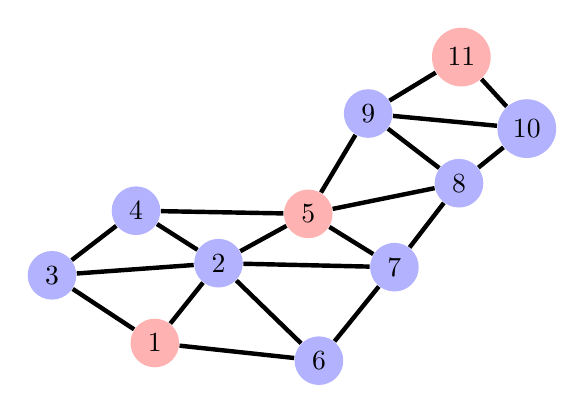
\begin{tikzpicture}
      \node (n1) at (1.108060,0.168294)  [circle,fill=red!30]  {1};
\node (n2) at (1.916771,1.181859)  [circle,fill=blue!30] {2};
\node (n3) at (-0.197998,1.028224) [circle,fill=blue!30] {3};
\node (n4) at (0.869271,1.848640)  [circle,fill=blue!30] {4};
\node (n5) at (3.056732,1.808215)  [circle,fill=red!30]  {5};
\node (n6) at (3.192034,-0.055883) [circle,fill=blue!30] {6};
\node (n7) at (4.150780,1.131397)  [circle,fill=blue!30] {7};
\node (n8) at (4.970900,2.197872)  [circle,fill=blue!30] {8};
\node (n9) at (3.817774,3.082424)  [circle,fill=blue!30] {9};
\node (n10) at (5.832186,2.891196) [circle,fill=blue!30] {10};
\node (n11) at (5.000885,3.800002) [circle,fill=red!30]  {11};
\draw[ultra thick] (n1) -- (n2);
\draw[ultra thick] (n1) -- (n3);
\draw[ultra thick] (n1) -- (n6);
\draw[ultra thick] (n2) -- (n3);
\draw[ultra thick] (n2) -- (n4);
\draw[ultra thick] (n2) -- (n5);
\draw[ultra thick] (n2) -- (n6);
\draw[ultra thick] (n2) -- (n7);
\draw[ultra thick] (n3) -- (n4);
\draw[ultra thick] (n4) -- (n5);
\draw[ultra thick] (n5) -- (n7);
\draw[ultra thick] (n5) -- (n8);
\draw[ultra thick] (n5) -- (n9);
\draw[ultra thick] (n6) -- (n7);
\draw[ultra thick] (n7) -- (n8);
\draw[ultra thick] (n8) -- (n9);
\draw[ultra thick] (n8) -- (n10);
\draw[ultra thick] (n9) -- (n10);
\draw[ultra thick] (n9) -- (n11);
\draw[ultra thick] (n10) -- (n11);


    \end{tikzpicture}
  \end{center}
  
  \begin{itemize}
  \item Start with $S$ empty
  \item For each $v \in V$ {\em sequentially}, add $v$ to $S$ if possible.
  \end{itemize}

\end{frame}


\begin{frame}
  \frametitle{Luby's algorithm}

  \begin{itemize}
  \item Init $S := \emptyset$
  \item Init candidates $C := V$
  \item While $C \neq \emptyset$
    \begin{itemize}
    \item Label each $v$ with a random $r(v)$
    \item For each $v \in C$ in parallel, if $r(v) <
      \min_{\mathcal{N}(v)} r(u)$
      \begin{itemize}
      \item Move $v$ from $C$ to $S$
      \item Remove neighbors from $v$ to $C$
      \end{itemize}
    \end{itemize}
  \end{itemize}
  Very probably finishes in $O(\log n)$ rounds.
\end{frame}


\begin{frame}
  \frametitle{Luby's algorithm (round 1)}

  \begin{center}
    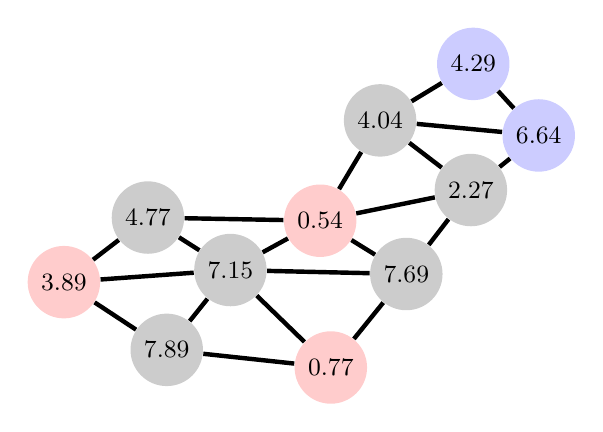
\begin{tikzpicture}
      \node (n1) at (1.108060,0.168294) [circle,fill=black!20] {\small 7.89};
\node (n2) at (1.916771,1.181859) [circle,fill=black!20] {\small 7.15};
\node (n3) at (-0.197998,1.028224) [circle,fill=red!20] {\small 3.89};
\node (n4) at (0.869271,1.848640) [circle,fill=black!20] {\small 4.77};
\node (n5) at (3.056732,1.808215) [circle,fill=red!20] {\small 0.54};
\node (n6) at (3.192034,-0.055883) [circle,fill=red!20] {\small 0.77};
\node (n7) at (4.150780,1.131397) [circle,fill=black!20] {\small 7.69};
\node (n8) at (4.970900,2.197872) [circle,fill=black!20] {\small 2.27};
\node (n9) at (3.817774,3.082424) [circle,fill=black!20] {\small 4.04};
\node (n10) at (5.832186,2.891196) [circle,fill=blue!20] {\small 6.64};
\node (n11) at (5.000885,3.800002) [circle,fill=blue!20] {\small 4.29};
\draw[ultra thick] (n1) -- (n2);
\draw[ultra thick] (n1) -- (n3);
\draw[ultra thick] (n1) -- (n6);
\draw[ultra thick] (n2) -- (n3);
\draw[ultra thick] (n2) -- (n4);
\draw[ultra thick] (n2) -- (n5);
\draw[ultra thick] (n2) -- (n6);
\draw[ultra thick] (n2) -- (n7);
\draw[ultra thick] (n3) -- (n4);
\draw[ultra thick] (n4) -- (n5);
\draw[ultra thick] (n5) -- (n7);
\draw[ultra thick] (n5) -- (n8);
\draw[ultra thick] (n5) -- (n9);
\draw[ultra thick] (n6) -- (n7);
\draw[ultra thick] (n7) -- (n8);
\draw[ultra thick] (n8) -- (n9);
\draw[ultra thick] (n8) -- (n10);
\draw[ultra thick] (n9) -- (n10);
\draw[ultra thick] (n9) -- (n11);
\draw[ultra thick] (n10) -- (n11);

    \end{tikzpicture}
  \end{center}
\end{frame}


\begin{frame}
  \frametitle{Luby's algorithm (round 1)}

  \begin{center}
    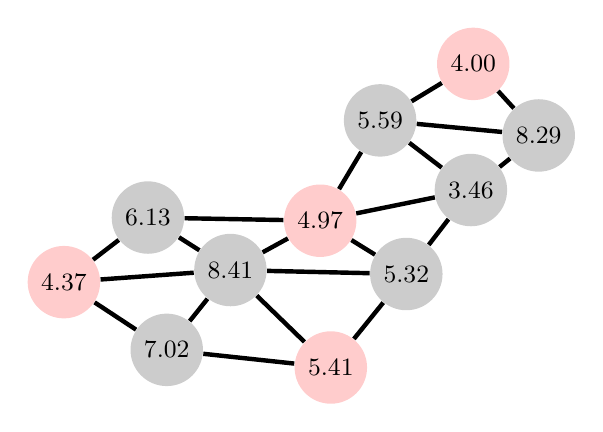
\begin{tikzpicture}
      \node (n1) at (1.108060,0.168294) [circle,fill=black!20] {\small 7.02};
\node (n2) at (1.916771,1.181859) [circle,fill=black!20] {\small 8.41};
\node (n3) at (-0.197998,1.028224) [circle,fill=red!20] {\small 4.37};
\node (n4) at (0.869271,1.848640) [circle,fill=black!20] {\small 6.13};
\node (n5) at (3.056732,1.808215) [circle,fill=red!20] {\small 4.97};
\node (n6) at (3.192034,-0.055883) [circle,fill=red!20] {\small 5.41};
\node (n7) at (4.150780,1.131397) [circle,fill=black!20] {\small 5.32};
\node (n8) at (4.970900,2.197872) [circle,fill=black!20] {\small 3.46};
\node (n9) at (3.817774,3.082424) [circle,fill=black!20] {\small 5.59};
\node (n10) at (5.832186,2.891196) [circle,fill=black!20] {\small 8.29};
\node (n11) at (5.000885,3.800002) [circle,fill=red!20] {\small 4.00};
\draw[ultra thick] (n1) -- (n2);
\draw[ultra thick] (n1) -- (n3);
\draw[ultra thick] (n1) -- (n6);
\draw[ultra thick] (n2) -- (n3);
\draw[ultra thick] (n2) -- (n4);
\draw[ultra thick] (n2) -- (n5);
\draw[ultra thick] (n2) -- (n6);
\draw[ultra thick] (n2) -- (n7);
\draw[ultra thick] (n3) -- (n4);
\draw[ultra thick] (n4) -- (n5);
\draw[ultra thick] (n5) -- (n7);
\draw[ultra thick] (n5) -- (n8);
\draw[ultra thick] (n5) -- (n9);
\draw[ultra thick] (n6) -- (n7);
\draw[ultra thick] (n7) -- (n8);
\draw[ultra thick] (n8) -- (n9);
\draw[ultra thick] (n8) -- (n10);
\draw[ultra thick] (n9) -- (n10);
\draw[ultra thick] (n9) -- (n11);
\draw[ultra thick] (n10) -- (n11);

    \end{tikzpicture}
  \end{center}
\end{frame}


\begin{frame}
  \frametitle{A fundamental problem}

  Many graph ops are
  \begin{itemize}
  \item Computationally cheap (per node or edge)
  \item Bad for locality
  \end{itemize}
  {\bf Memory bandwidth} as a limiting factor.
\end{frame}

\begin{frame}
  \frametitle{Big data?}

  Consider:
  \begin{itemize}
  \item 323 million in US (fits in 32-bit int)
  \item About 350 Facebook friends each
  \item Compressed sparse row: about 450 GB
  \end{itemize}
  Topology (no metadata) on one big cloud node...
\end{frame}

\begin{frame}
  \frametitle{Graph representation: Adjacency matrix}

  \begin{center}
    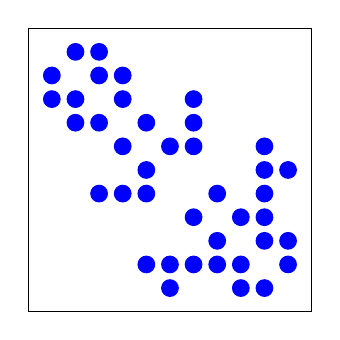
\begin{tikzpicture}
      \draw (-0.3,0) rectangle (3.300000,3.600000);
\filldraw[blue] (3.000000,0.600000) circle (3pt);
\filldraw[blue] (3.000000,0.900000) circle (3pt);
\filldraw[blue] (3.000000,1.800000) circle (3pt);
\filldraw[blue] (2.700000,0.300000) circle (3pt);
\filldraw[blue] (2.700000,0.900000) circle (3pt);
\filldraw[blue] (2.700000,1.200000) circle (3pt);
\filldraw[blue] (2.700000,1.500000) circle (3pt);
\filldraw[blue] (2.700000,1.800000) circle (3pt);
\filldraw[blue] (2.700000,2.100000) circle (3pt);
\filldraw[blue] (2.400000,0.300000) circle (3pt);
\filldraw[blue] (2.400000,0.600000) circle (3pt);
\filldraw[blue] (2.400000,1.200000) circle (3pt);
\filldraw[blue] (2.100000,0.600000) circle (3pt);
\filldraw[blue] (2.100000,0.900000) circle (3pt);
\filldraw[blue] (2.100000,1.500000) circle (3pt);
\filldraw[blue] (1.800000,0.600000) circle (3pt);
\filldraw[blue] (1.800000,1.200000) circle (3pt);
\filldraw[blue] (1.800000,2.100000) circle (3pt);
\filldraw[blue] (1.800000,2.400000) circle (3pt);
\filldraw[blue] (1.800000,2.700000) circle (3pt);
\filldraw[blue] (1.500000,0.300000) circle (3pt);
\filldraw[blue] (1.500000,0.600000) circle (3pt);
\filldraw[blue] (1.500000,2.100000) circle (3pt);
\filldraw[blue] (1.200000,0.600000) circle (3pt);
\filldraw[blue] (1.200000,1.500000) circle (3pt);
\filldraw[blue] (1.200000,1.800000) circle (3pt);
\filldraw[blue] (1.200000,2.400000) circle (3pt);
\filldraw[blue] (0.900000,1.500000) circle (3pt);
\filldraw[blue] (0.900000,2.100000) circle (3pt);
\filldraw[blue] (0.900000,2.700000) circle (3pt);
\filldraw[blue] (0.900000,3.000000) circle (3pt);
\filldraw[blue] (0.600000,1.500000) circle (3pt);
\filldraw[blue] (0.600000,2.400000) circle (3pt);
\filldraw[blue] (0.600000,3.000000) circle (3pt);
\filldraw[blue] (0.600000,3.300000) circle (3pt);
\filldraw[blue] (0.300000,2.400000) circle (3pt);
\filldraw[blue] (0.300000,2.700000) circle (3pt);
\filldraw[blue] (0.300000,3.300000) circle (3pt);
\filldraw[blue] (0.000000,2.700000) circle (3pt);
\filldraw[blue] (0.000000,3.000000) circle (3pt);

    \end{tikzpicture}

    Pro: efficient for dense graphs \\
    Con: wasteful for sparse case...
  \end{center}
\end{frame}

\begin{frame}
  \frametitle{Graph representation: Coordinate}

  \begin{itemize}
  \item Tuples: $(i,j,w_{ij})$
  \item Pro: Easy to update
  \item Con: Slow for multiply
  \end{itemize}
\end{frame}

\begin{frame}
  \frametitle{Graph representation: Adj list}

  \begin{itemize}
  \item Linked lists of adjacent nodes
  \item Pro: Still easy to update
  \item Con: May cost more to store than coord?
  \end{itemize}
\end{frame}

\begin{frame}
  \frametitle{Graph representations: CSR}
  
  \begin{center}
    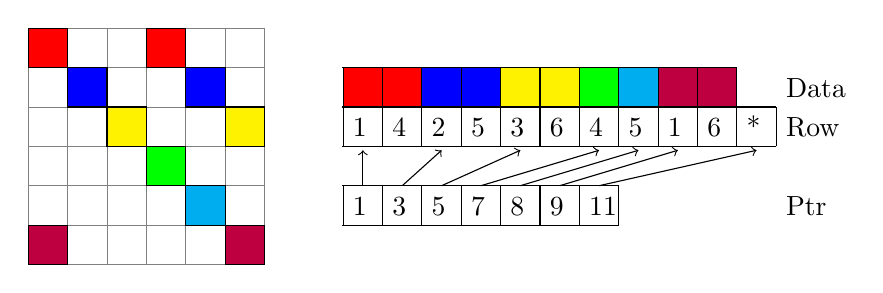
\begin{tikzpicture}
  \draw[step=0.5,gray,very thin] (-1,0) grid (2.0,3.0);
  \draw[fill=red]    (-1.0,2.5) rectangle (-0.5,3.0);
  \draw[fill=red]    ( 0.5,2.5) rectangle ( 1.0,3.0);
  \draw[fill=blue]   (-0.5,2.0) rectangle ( 0.0,2.5);
  \draw[fill=blue]   ( 1.0,2.0) rectangle ( 1.5,2.5);
  \draw[fill=yellow] ( 0.0,1.5) rectangle ( 0.5,2.0);
  \draw[fill=yellow] ( 1.5,1.5) rectangle ( 2.0,2.0);
  \draw[fill=green]  ( 0.5,1.0) rectangle ( 1.0,1.5);
  \draw[fill=cyan]   ( 1.0,0.5) rectangle ( 1.5,1.0);
  \draw[fill=purple] ( 1.5,0.0) rectangle ( 2.0,0.5);
  \draw[fill=purple] (-1.0,0.0) rectangle (-0.5,0.5);

  \draw[fill=red]    (3.0,2.0) rectangle (4.0,2.5);
  \draw[fill=blue]   (4.0,2.0) rectangle (5.0,2.5);
  \draw[fill=yellow] (5.0,2.0) rectangle (6.0,2.5);
  \draw[fill=green]  (6.0,2.0) rectangle (6.5,2.5);
  \draw[fill=cyan]   (6.5,2.0) rectangle (7.0,2.5);
  \draw[fill=purple] (7.0,2.0) rectangle (8.0,2.5);
  
  \draw[step=0.5,black] (2.99,2.0) grid (8.0,2.5);
  \draw[step=0.5,black] (2.99,1.499) grid (8.5,2.0);
  \draw[step=0.5,black] (2.99,0.499) grid (6.5,1.0);

  \draw (3.0,1.5) node[anchor=south west] {1};
  \draw (3.5,1.5) node[anchor=south west] {4};
  \draw (4.0,1.5) node[anchor=south west] {2};
  \draw (4.5,1.5) node[anchor=south west] {5};
  \draw (5.0,1.5) node[anchor=south west] {3};
  \draw (5.5,1.5) node[anchor=south west] {6};
  \draw (6.0,1.5) node[anchor=south west] {4};
  \draw (6.5,1.5) node[anchor=south west] {5};
  \draw (7.0,1.5) node[anchor=south west] {1};
  \draw (7.5,1.5) node[anchor=south west] {6};
  \draw (8.0,1.5) node[anchor=south west] {*};

  \draw (3.0,0.5) node[anchor=south west] {1};
  \draw (3.5,0.5) node[anchor=south west] {3};
  \draw (4.0,0.5) node[anchor=south west] {5};
  \draw (4.5,0.5) node[anchor=south west] {7};
  \draw (5.0,0.5) node[anchor=south west] {8};
  \draw (5.5,0.5) node[anchor=south west] {9};
  \draw (6.0,0.5) node[anchor=south west] {11};

  \draw [->] (3.25,1.0) -- (3.25,1.45); % 1
  \draw [->] (3.75,1.0) -- (4.25,1.45); % 3
  \draw [->] (4.25,1.0) -- (5.25,1.45); % 5
  \draw [->] (4.75,1.0) -- (6.25,1.45); % 7
  \draw [->] (5.25,1.0) -- (6.75,1.45); % 8
  \draw [->] (5.75,1.0) -- (7.25,1.45); % 9
  \draw [->] (6.25,1.0) -- (8.25,1.45);

  \draw (8.5,2.0) node[anchor=south west] {Data};
  \draw (8.5,1.5) node[anchor=south west] {Row};
  \draw (8.5,0.5) node[anchor=south west] {Ptr};
\end{tikzpicture}


    Pro: traversal?  Con: updates
  \end{center}  
\end{frame}

\begin{frame}
  \frametitle{Graph representations: implicit}

  \begin{itemize}
  \item Idea: Never materialize a graph data structure
  \item Key: Provide traversal primitives
  \item Pro: Explicit rep'n sometimes overkill for one-off graphs?
  \item Con: Hard to use canned software (except NLA?)
  \end{itemize}
\end{frame}

\begin{frame}
  \frametitle{Graph algorithms and linear algebra}

  \begin{itemize}
  \item Looks like LA
    \begin{itemize}
    \item Floyd-Warshall
    \item Breadth-first search?
    \end{itemize}
  \item Really is standard LA
    \begin{itemize}
    \item Spectral partitioning and clustering
    \item PageRank and some other centralities
    \item ``Laplacian Paradigm'' (Spielman, Teng, others...)
    \end{itemize}
  \end{itemize}
\end{frame}

\begin{frame}
  \frametitle{Graph algorithms and linear algebra}

  {\em Semirings} have $\oplus$ and $\otimes$ s.t.
  \begin{itemize}
  \item Addition is commutative+associative with an identity 0
  \item Multiplication is associative with identity 1
  \item Both are distributive
  \item $a \otimes 0 = 0 \otimes a = 0$
  \item But no subtraction or division
  \end{itemize}
  Technically have {\em modules} (vs vector spaces) over semirings
\end{frame}

\begin{frame}
  \frametitle{Graph algorithms and linear algebra}

  Example: min-plus
  \begin{itemize}
  \item $\oplus = \min$ and additive identity $0 \equiv \infty$
  \item $\otimes = +$ and multiplicative identity $1 \equiv 0$
  \item Useful for breadth-first search (on board)
  \end{itemize}
  
\end{frame}

\begin{frame}
  \frametitle{Graph BLAS}

  \begin{center}
    \url{http://www.graphblas.org/}
  \end{center}
  \begin{itemize}
  \item Provisional API as of late May 2017
  \item (Opaque) internal sparse matrix data structure
  \item Allows operations over misc semirings
  \end{itemize}
\end{frame}

\begin{frame}
  \frametitle{Graph frameworks}

  Several to choose from!
  \begin{itemize}
  \item Pregel, Apache Giraph, Stanford GPS, ...
  \item GraphLab family
    \begin{itemize}
    \item GraphLab: Original distributed memory
    \item PowerGraph: Tuned toward ``natural'' (power law) networks
    \item GraphChi: {\em Chi}huahua -- shared memory vs distributed
    \end{itemize}
  \item Outperformed by Galois, Ligra, BlockGRACE, others
  \item But... programming model was easy
  \end{itemize}
\end{frame}

\begin{frame}
  \frametitle{Graph frameworks}

  \begin{itemize}
  \item ``Think as a vertex''
    \begin{itemize}
    \item Each vertex updates locally
    \item Exchanges messages with neighbors
    \item Runtime actually schedules updates/messages
    \end{itemize}
  \item Message sent at super-step $S$ arrives at $S+1$
  \item Looks like BSP
  \end{itemize}
\end{frame}

\begin{frame}
  \frametitle{At what COST?}

  \begin{center}
    ``Scalability!  But at what COST?'' \\
    McSherry, Isard, Murray \\
    HotOS 15
  \end{center}

  \begin{quote}
    You can have a second computer once you've shown you know how to
    use the first one. \\ \hfill -- Paul Barham (quoted in intro to
    HotOS15 paper)
  \end{quote}
  \begin{itemize}
  \item COST = Configuration that Outperforms a Single Thread
  \item Observation: many systems have unbounded COST!
  \end{itemize}
\end{frame}

\end{document}
